\RequirePackage[l2tabu,orthodox]{nag}
\documentclass[11pt,letterpaper]{article}
\usepackage[T1]{fontenc}
\usepackage[utf8]{inputenc}
\usepackage{crimson}
\usepackage{helvet}
\usepackage[strict,autostyle]{csquotes}
\usepackage[USenglish]{babel}
\usepackage{microtype}
\usepackage{authblk}
\usepackage{booktabs}
\usepackage{caption}
\usepackage{endnotes}
\usepackage{geometry}
\usepackage{graphicx}
\usepackage{hyperref}
\usepackage{natbib}
\usepackage{rotating}
\usepackage{setspace}
\usepackage{titlesec}
\usepackage{url}
\usepackage{soul}
\usepackage[dvipsnames]{xcolor}
\usepackage[many]{tcolorbox}
\newtcolorbox{mybox}{colback = black!5!gray!50, colframe = black!75!black, segmentation style={solid}} % create text box
\usepackage{hanging}

% location of figure files, via graphicx package
\graphicspath{{./figures/}}

% configure the page layout, via geometry package
\geometry{
	paper=letterpaper,
	top=2.5cm,
	bottom=2.5cm,
	left=2.5cm,
	right=2.5cm}
\setstretch{1.02}
\clubpenalty=10000
\widowpenalty=10000

% set section/subsection headings as the sans serif font
\titleformat{\section}{\normalfont\sffamily\large\bfseries}{\thesection.}{0.3em}{}
\titleformat{\subsection}{\normalfont\sffamily\small\bfseries}{\thesubsection.}{0.3em}{}

% make figure/table captions sans-serif small font
\captionsetup{font={footnotesize,sf},labelfont=bf,labelsep=period}

% configure pdf metadata and link handling
\hypersetup{
	pdfauthor={Carmen Cabrera-Arnau},
	pdftitle={The mid-term impact of COVID-19 on human mobility patterns in Latin American countries},
	pdfsubject={Title},
	pdfkeywords={Keywords},
	pdffitwindow=true,
	breaklinks=true,
	colorlinks=false,
	pdfborder={0 0 0}}

\title{The mid-term impact of COVID-19 on human mobility patterns in Latin American countries\footnote{\textbf{Citation}: Cabrera-Arnau, C., González-Leonardo, M., Nasuto, A., Neville, R., Rowe, F. (2023). The mid-term impact of COVID-19 on human mobility patterns in Latin American countries}}
\author[1]{Carmen Cabrera-Arnau \thanks{\textit{Corresponding author}: c.cabrera-arnau@liverpool.ac.uk}}
\author[2]{Miguel González-Leonardo}
\author[1]{Andrea Nasuto}
\author[1]{Ruth Neville}
\author[1]{Francisco Rowe}
\affil[1]{Geographic Data Science Lab, Department of Geography and Planning, University of Liverpool, Liverpool, United Kingdom}
\affil[2]{Center for Demographic, Urban and Environmental Studies, El Colegio de México (COLMEX), Mexico City, Mexico}

\date{}

% From pandoc:
% https://github.com/jgm/pandoc-templates/blob/master/default.latex
\newlength{\cslhangindent}
\setlength{\cslhangindent}{1.5em}
\newlength{\csllabelwidth}
\setlength{\csllabelwidth}{3em}
\newlength{\cslentryspacingunit} % times entry-spacing
\setlength{\cslentryspacingunit}{\parskip}
\newenvironment{CSLReferences}[2] % #1 hanging-ident, #2 entry spacing
 {% don't indent paragraphs
  \setlength{\parindent}{0pt}
  % turn on hanging indent if param 1 is 1
  \ifodd #1
  \let\oldpar\par
  \def\par{\hangindent=\cslhangindent\oldpar}
  \fi
  % set entry spacing
  \setlength{\parskip}{#2\cslentryspacingunit}
 }%
 {}
\usepackage{calc}
\newcommand{\CSLBlock}[1]{#1\hfill\break}
\newcommand{\CSLLeftMargin}[1]{\parbox[t]{\csllabelwidth}{#1}}
\newcommand{\CSLRightInline}[1]{\parbox[t]{\linewidth - \csllabelwidth}{#1}\break}
\newcommand{\CSLIndent}[1]{\hspace{\cslhangindent}#1}
\setlength{\emergencystretch}{3em} % prevent overfull lines
\providecommand{\tightlist}{%
  \setlength{\itemsep}{0pt}\setlength{\parskip}{0pt}}

% https://stackoverflow.com/questions/41052687/rstudio-pdf-knit-fails-with-environment-shaded-undefined-error


\begin{document}

\maketitle


\begin{abstract}

Recent empirical studies, predominantly from countries in the Global North, have shown that the COVID-19 pandemic disrupted human mobility at different spatial scales, but particularly in big cities, initially identified as epicentres of infections. Lockdowns, remote work, and online education decreased the demand for commuting and urban living, resulting in an "urban exodus". Despite the existing evidence, little is known about whether counterurbanisation movements have unfolded similarly in the Global South. In this study, we use anonymised, high-resolution location data from Facebook users to answer the following research questions: i) to what extent are people leaving cities? ii) are there variations across countries? iii) are there changes in mobility patterns over time? iv) how long do these changes last? The methodology involves three steps. Firstly, we quantify the number of movements between different locations in each country. Second, we use statistical modelling and spatial interaction models to assess the strength of the flows between specific origin-destination pairs at different points in time. Thirdly, for each country, we use cluster analysis to characterise different mobility behaviours according to the population density at the origin and the destination. We obtain population density data from Worldpop at a resolution of 1 sqkm, and we use it as a proxy of the level of urbanisation at these locations. 

%\vspace{1cm}
\end{abstract}



\pagebreak

\section{Introduction}

The COVID-19 pandemic globally resulted in disruptive shocks to the
human mobility system. Governments stringency measures and the economic
downturn caused by the pandemic constrained international migration
(\textbf{internat2021?}; \textbf{gonzález-leonardo2022?};
\textbf{gonzález-leonardo2023?}) and population movements within
countries (\textbf{nouvellet2021?}; \textbf{gonzález-leonardo2022a?};
Wang et al. 2022; \textbf{rowe2023?}). During early stages of the
pandemic, big cities became the main epicentres of COVID-19 infections
and deaths (\textbf{Pomeroy2021?}) due to their higher connectivity via
air travel, higher population density and concentration of public-facing
jobs (\textbf{brandén2020?}; \textbf{bhadra2020?}). As a result,
governments implemented non-pharmaceutical interventions, such as
lockdowns and business closures, leading to increases in unemployment
and removing the urban vibrancy (\textbf{blustein2020?};
\textbf{BBCnews2023?}). In addition, remote work and online teaching
reduced the need for commuting, living close to work and education
centers, and added pressure for individuals living in small and crowded
spaces to move out of cities and look for more affordable and
comfortable housing (\textbf{nathan2020?}; \textbf{USBureauLabor2021?}).
These changes are believed to have reduced the attractiveness of cities
during the pandemic, while suburbs and rural areas have gained
popularity (\textbf{florida2021?}). As a result, a number of headlines
have claimed the emergence of an `urban exodus' to areas with lower
population densities (e.g. (\textbf{TheGuardian2020?})).

Despite their potential rise in popularity, remote locations offer
limited availability and diversity of job opportunities, and tend to
lack infrastructure and services, such as schooling and health, to
effectively accommodate a large population influx
(\textbf{Pinilla2021?}; \textbf{oecdreg?}). They generally lack
high-speed Internet connection which is vital for teleworking
(\textbf{Chen2004?}). Additionally, most jobs cannot be done remotely
(\textbf{oecdsoc?}), and some companies have returned to in-person
office work or have implemented hybrid forms of work, following the
relaxation of stringency measures (\textbf{McKinsey21?}). Schools and
universities have also returned to face-to-face teaching. Therefore,
living close to work or study places remains relevant. Businesses and
leisure activities in cities have gradually returned to normal,
reinvigorating the economic functioning and urban life. Collectively,
these arguments suggest that a potential increase in counterurbanisation
movements during the pandemic was concentrated during periods of
stringency measures and is likely to be short term. Big cities have
successfully weathered previous pandemics (\textbf{huremovic2019?};
\textbf{Glaeser20?}) and are likely to remain attractive places to live.
Thanks to agglomeration economies, cities are normally regarded as
centres for economic growth, clusters of talent, consumer bases and
spaces for face‐to‐face interaction and diversity
(\textbf{storper2004?}; \textbf{florida2021?}).

Recent empirical evidence has shown a decline on human mobility during
periods of severe stringency measures, coupled with a rise of movements
from cities to less populated areas and a slowdown of urbanisation
movements across some countries of the Global North: the United States
(\textbf{ramani2021?}), United Kingdom (\textbf{rowe2023?}; Wang et al.
2022), Spain (\textbf{gonzález-leonardo2022b?};
\textbf{gonzález-leonardo2022a?}), Germany {[}@;
(\textbf{stawarz2022?}){]}, Sweden (\textbf{vogiazides2022?}), Norway
(\textbf{tønnessen2021?}), Australia (\textbf{perales2022?}) and Japan
(\textbf{kotsubo2022?}). The majority of movements away from cities
headed to their suburbs (\textbf{vogiazides2022?};
\textbf{stawarz2022?}) or rural areas in their close proximity
(\textbf{gonzález-leonardo2022b?}; \textbf{gonzález-leonardo2022a?})
showing in some instances a ``doghnut effect'', with a decline in
population movements directed to cities and a rise in the inflow of
people to less dense surrounding areas (\textbf{ramani2021?}). Studies
demonstrated that professionals (\textbf{tønnessen2021?}) and
individuals with a high income (\textbf{haslag2021?}), those who are
potentially able to practice remote working, underpinned movements away
from large cities. In addition, research has shown that a large share of
counterurbanisation movements is headed to touristic locations with a
high concentration of second homes, suggesting that middle and high
class individuals may have been key actors in movements from cities to
less populated areas during the pandemic
(\textbf{gonzález-leonardo2022a?}). However, most studies suggested that
variations in internal population movements during the pandemic are
likely to be temporary and have not altered previous macro-structures of
human mobility across the rural-urban hierarchy (\textbf{rowe2023?}).

In Latin America and the Caribbean, a reduction in internal population
movements was documented during periods of high stringency
(\textbf{aromí2023?}), but there is no evidence on how human mobility
has changed across the rural-urban continuum. Anecdotal reports have
shown that movements away from cities seem to have accelerated in two
countries of the Global South, India (\textbf{irudayarajan2020?}) and
South Africa (\textbf{ginsburg2022?}), while urbanisation trends have
decelerated. However, lack of suitable up-to-date data has prevented us
from properly assessing the ``urban exodus'' hypothesis in Global South
countries, as well as the extent, spatial patterns, and durability of
potential changes on internal population movements. The evidence for
these two countries suggested that increasing counterurbanisation
movements during the pandemic in India and South Africa could be
underpinned by internal migrants residing in cities who returned to
their hometowns due to a rise in unemployment
(\textbf{irudayarajan2020?}; \textbf{ginsburg2022?}). However, recent
studies have shown that urban residents from wealthy neighborhoods were
more likely to move to rural areas than those from low income
neighborhoods during the first wave of the pandemic in Brazil, Colombia,
Mexico, Indonesia, Philippines and South Africa
(\textbf{lucchini2023?}).

It is known that human mobility within countries tends to vary in
systematic ways with development levels (\textbf{bell2015?}). In Latin
America and the Caribbean, 28.6\% of the population was living on less
than \$6.8 per day in 2020 (\textbf{WorldBank2023?}) and the informality
rate was about 53\% in 2016 (\textbf{OIT2018?}). Thus, we could expect
different pandemic impacts on the patterns of internal population
movements between countries in the Global North and the Global South.
The way in which COVID-19 unfolded in each country, with varying levels
of stringency measures, may have also produced different outcomes on
human mobility.

Traditionally, censuses have been used to analyse human mobility
patterns within Global South countries, which lack register data
(\textbf{bell2015?}; \textbf{bernard2017?}). Censuses, however, are
normally updated every 10 years, lacking the temporal granularity to
explore population movements over yearly, monthly or short-time
intervals.

Digital traces data from mobile phone applications, on the other hand,
provide a unique opportunity to capture internal population movements
with small spatial and temporal granularity in multiple countries
(\textbf{green2021?}; \textbf{rowe2021?}). Drawing on geographically
granular Meta-Facebook data from March 2020 to March 2022, we aim to
analyse how the pandemic has changed the patterns of human mobility
across the rural-urban hierarchy in four Latin American countries:
Argentina, Chile, Colombia and Mexico. We aim to address the following
research questions: 1) To what extent did people leave cities and move
to less populated areas in these countries? 2) Which are the spatial
patterns of potential changes on internal population movements? 3) How
have the patterns of human mobility changed over the course of the
pandemic? 4) Are potential changes likely to endure the pandemic?

The rest of the paper is structured as follows: \ldots{}

\section{Background}

\subsection{What do we know about internal population movements during the pandemic?}

The COVID-19 pandemic led to an overall decline in human mobility within
countries (\textbf{nouvellet2021?}). Research has shown that internal
population movements across the rural-urban continuum decreased in the
United States (\textbf{ramani2021?}), several European countries, Japan
and Austria during 2020 (\textbf{rowe2023?}). Declines ranged from 2.5\%
in Spain to 8.5\% in Australia. The largest drops occurred during
periods of national lockdowns and the implementation of other stringency
measures, such as mobility restrictions, work and school closing, while
levels of internal population movements recovered or exceeded
pre-pandemic figures when lockdowns were lifted. Declines were partially
attributed to a reduction in involuntary migration during lockdowns, a
loss of labour market dynamism due to the pandemic, fewer people
changing jobs and increasing remote work (\textbf{perales2022?}).

COVID-19 has also altered patterns of internal population movements
across the rural-urban hierarchy (Rowe et al. 2022). In large metro
areas across the United States, population movements, as well as
households and businesses, shifted from central cities to suburbs and
exurbs during 2020 (\textbf{ramani2021?}). These authors label this
trend as a ``doughnut effect'', reflecting a decrease in population
inflows and activities in city centers and a growth in suburban rings.
They found a sizeable ``doghnut effect'' in large cities, a smaller
effect in medium-sized cities and almost no effect for small cities. A
similar trend was observed in Norway (\textbf{tønnessen2021?}), Germany
(\textbf{stawarz2022?}), Sweden (\textbf{vogiazides2022?}) and Japan
(\textbf{fielding2021?}; \textbf{kotsubo2022?}), where net migration
rates in big cities declined, while population movement to their suburbs
increased. In addition, this trend was accompanied by a deceleration of
urbanisation trends and unusual population gains in rural areas due to
an acceleration in counterurbanisation movements, mostly in rural
locations which are known to be holiday destinations with a high
concentration of second homes and are generally located in the close
proximity to big cities. An increase of counterurbanisation was the main
pandemic outcome on human mobility in Spain
(\textbf{gonzález-leonardo2022b?}; \textbf{gonzález-leonardo2022a?}),
the United Kingdom (Wang et al. 2022; Rowe et al. 2022) and Australia
(\textbf{perales2022?}), where there is no evidence of a ``doghnut
effect'', since substantial variations in suburbs were not found across
these countries.

However, studies suggest that variations are likely to be temporary
(\textbf{rowe2023?}). In Spain, the urbanisation movement returned to
pre-pandemic levels when the lockdown ended in mid-June 2020
(\textbf{gonzález-leonardo2022b?}) and unusually high levels of
counterurbanisation persisted over 2021, although the majority of
movements continued to occur between and within urban areas
(\textbf{gonzález-leonardo2022a?}). In Australia, the pandemic has
caused minor changes in spatial patterns of internal migration, and its
effects were minimal by the end of 2020 (\textbf{perales2022?}). In the
United Kingdom, mobility patterns returned to those registered prior to
the pandemic after the easing of non-pharmaceutical interventions (Rowe
et al. 2022; Wang et al. 2022). These findings suggest that COVID-19
generated shock waves leading to temporary changes in the patterns of
internal population movement across the rural-urban continuum, but it
has not significantly altered the prevalent macro-structures of
population movement within countries.

Despite some evidence in the Global North, lees is known about the
impact of COVID-19 on human mobility in the Global South countries. In
Latin America and the Caribbean, internal population movements declined
by 10\% during periods of severe stringent measures, from 16-19\% in
Bolivia, Ecuador and Argentina to less than 3\% in Paraguay and
Venezuela (\textbf{aromí2023?}). However, there is no evidence about
pandemic outcomes on human mobility across the rural-urban continuum. To
date, surveys carried out in India (\textbf{irudayarajan2020?}) and
South Africa (\textbf{ginsburg2022?}) have shown anecdotal evidence
suggesting that urbanisation trends declined during the pandemic, while
movements from cities to rural areas increased. Both studies pointed out
that a number of rural residents initiating a migration decreased during
2020 and some labourers in major cities seem to have returned to their
hometowns due to job losses, since stringency measures have extensively
impacted the functioning of the economy (\textbf{ghosh2020?}). Many
internal migrants residing in Indian cities lost their jobs and were
unable to afford basic necessities (\textbf{ILO2020?}). Collectively,
these findings suggest that vulnerable populations seem to have played a
role in increasing counterurbanisation movements in Global South
countries. However, recent work has shown that high-wealth groups
residing in cities across Mexico, Colombia, Brazil, Indonesia,
Philippines and South Africa were on average 159\% more likely to have
moved to rural area compared to those of low-wealth groups during early
stages of the pandemic (\textbf{lucchini2023?}), in line with the
evidencee found for Global North countries.

Despite anecdotal evidence suggesting pandemic impacts on the patterns
of human mobility across the rural-urban hierarchy in the Global South,
lack of suitable data has not allowed us to identify and quantify the
magnitude of these impacts. In this paper, we use Meta-Facebook data to
provide evidence on the effect of the pandemic on the patterns of
internal population movements across four Latin American countries.

\subsection{Contemporary trends of human mobility across the rural-urban hierarchy in Latin America}

Until 1980, rural to urban migration dominated internal population
movements in Latin America with significant levels of population
redistribution, especially during the rapid industrialisation process
between the 1950s and 1970s when a critical mass of individuals moved
from villages and towns to urban areas (\textbf{firebaugh1979?};
\textbf{lattes95?}; \textbf{sobrino12?}). Urban growth due to internal
mobility was primarily concentrated in large urban centres resulting in
a significant population imbalance between the chief cities and other
settlements (\textbf{PintoDaCunha02?}; \textbf{lattes2017?}). As a
consequence, Latin America shows high rates of urbanisation with more
than 81\% of the population living in cities, the highest figure after
North America, and about 46\% of urban residents settled in cities with
more than 1 million inhabitants (\textbf{UNpopulation19?}).

Currently, internal population movements amongst cities dominate the
migratory system in Latin America, while rural to urban flows are of
less importance (\textbf{bernard2017?}; \textbf{rodríguez-vignoli2018?};
\textbf{UNpopulation19?}). According to the 2010 census round, 80\% of
internal migrants moved between cities
(\textbf{rodríguez-vignoli2018?}). Contrary to the period preceding the
1980s, medium-sizes cities (those between 500K and 1 million
inhabitants) experienced the highest net migration rates, while large
cities (\textgreater1 million) presented balanced rates and small cities
(\textgreater500K) lost individuals by internal population movements
(\textbf{rodríguez-vignoli2018?}). Changing patterns in human mobility
within Latin American countries were driven by a decline in internal
migration since the 1980s crisis (\textbf{chávezgalindo2016?}) and
deconcentration dynamics in large urban centres, such as Mexico City
(\textbf{sobrino2006?}) or Santiago de Chile
(\textbf{gonzálezollino2006?}), where long distance inflows have
declined over time. At the same time, there has been an increasing
domestic and foreign investment in export-oriented activities or tourism
industries in certain middle-sized cities, fostering the geographic
dispersal of employment opportunities and increasing the attractiveness
of these cities (\textbf{Brea03?}; \textbf{Pérez-Campuzano13?};
\textbf{chávezgalindo2016?}).

Suburbanisation also represents an important type of internal population
movement and has increased over time due to the growing expansion of
Latin American cities (\textbf{graizbord2007?};
\textbf{chávezgalindo2016?}). These movements are underpinned by flows
of middle- and upper-class families moving away from central cities to
surrounding auto-segregated areas of wealthy individuals
(\textbf{borsdorf2003?}; \textbf{rodríguezvignoli2017?}). Low-income
populations also settle in specific areas within suburbs where the cost
of living is usually cheaper than in cities (\textbf{janoschka2002?};
\textbf{rodríguezvignoli2017?}). A large proportion of both wealthy
individuals and low-income residents commute daily to central cities,
mainly for work reasons (\textbf{chávezgalindo2016?}). Recently,
reurbanisation dynamics have also been observed due to gentrification
processes in specific central areas (\textbf{sobrino12?};
\textbf{chávezgalindo2016?}). In this paper, we analyse how the COVID-19
pandemic has changed patterns of internal population movements across
the rural-urban hierarchy in Mexico, Colombia, Perú, Chile and
Argentina.

\section{Data}

The analysis proposed in this paper is based on several data sets.
Firstly, Facebook Population and Facebook Movements are data sets based
on the Facebook users' location history. The data sets were created by
Facebook's owner company Meta and can be accessed through their Data for
Good programme (\url{https://dataforgood.facebook.com/}). Prior to
releasing the data sets, Meta applies three techniques to ensure privacy
and anonymisation. First, a small undisclosed amount of random noise is
added to ensure that precise location cannot be identified for small
population counts in sparsely populated areas. While removing small
counts may lead to an underrepresentation of the population in these
places, the geographic distribution of population is still reflected in
the data. Second, spatial smoothing is applied to produce a smooth
population count surface using inverse distance-weighted averaging.
Third, any remaining population counts of less than 10 are removed from
the final data set (see Maas et al. Maas et al. (2019) for details).

Both data sets Facebook Population and Facebook Movements contain data
corresponding to a time period comprising approximately two years,
starting from March 2020, and to four Latin American countries,
Argentina, Chile, Colombia and Mexico. The data in both data sets is
temporally aggregated into three 8-hour windows (00:00--08:00,
08:00--16:00 and 16:00--00:00) for every day in the aforementioned
two-year period. It is spatially aggregated into tiles according to the
Bing Maps Tile System. This geospatial indexing system was developed by
Microsoft and it partitions the world into square cells at various
levels of resolution. The Facebook Movements and Facebook Population
datasets are aggregated into various levels of resolution depending on
the country, and the length of the Bing tile sides vary also by country
according to the country's distance to the Equator, even when two
countries use tiles at the same level of resolution.

The Facebook Population data set provides information on the number of
active Facebook users in each tile. The data set Facebook Movements
captures the total number of Facebook users moving between pairs of
origin and destination Bing tiles. We note here that due to the nature
of the Facebook Movement data, we cannot distinguish between different
types of movements, for example, daily commutes to work or permanent
changes of address. However, we are still able to detect the evolution
of movements between origin-destination pairs of Bing tiles and hence,
we are able to capture the impact that COVID-19 has on mobility
patterns.

On top of the data for the two-year period, each entry in the Facebook
Population and Facebook Movements datasets include data for baseline
levels before COVID-19. The baseline values are computed based on a
45-day period ending on the 10th of March of 2020. The data sets also
include a `quality' score indicating the number of standard deviations
by which the observed data at specific locations and time windows differ
from the baseline values, hence highlighting statistically significant
changes.

An additional data set from WorldPop was used to capture the spatial
distribution of population density in the different countries analysed
here. The WorlPop dataset is in raster format and contains gridded
population data at 1 sqkm resolution.

\section{Method}

\subsection{Data pre-processing}

Ultimately, we work with a dataset where each entry represents a
population flow between an origin and a destination pair. For each
entry, we consider when the movement took place, the population density
at the origin and destination, the number of active Facebook users at
the origin and destination and?

\subsubsection{Spatial aggregation}

The working dataset is aggregated at the same level as the Bing tiles
used to track the movements in a given country. To each Bing tile, we
aggregate WorldPop population data and use it to estimate the population
density of each Bing tile.

\subsubsection{Temporal aggregation}

The raw data is aggregated into 8-hour windows for every day in the
two-year period. However, we are interested in longer-term trends and
not in how population flows vary throughout the day. For this reason, we
obtain estimates for the parameters in the models described in
subsection \ref{subsec-models} by splitting the total data set by month.
For the visualisations in section \ref{sec-results}, we also present the
data aggregated by month.

\subsection{Classifying Bing tiles according to their population density}

Here we aim to understand how the population density at the origin and
the destination might influence mobility behaviours. To help
characterise the population density between orign and destination, we
classify the Bing tiles into 10 discrete categories of population
density according to the Jenks natural breaks classification method,
hence obtaining a categorisation of Bing tiles a lot more detailed than
the traditional binary rural/urban classification.

\begin{figure}[H]

{\centering 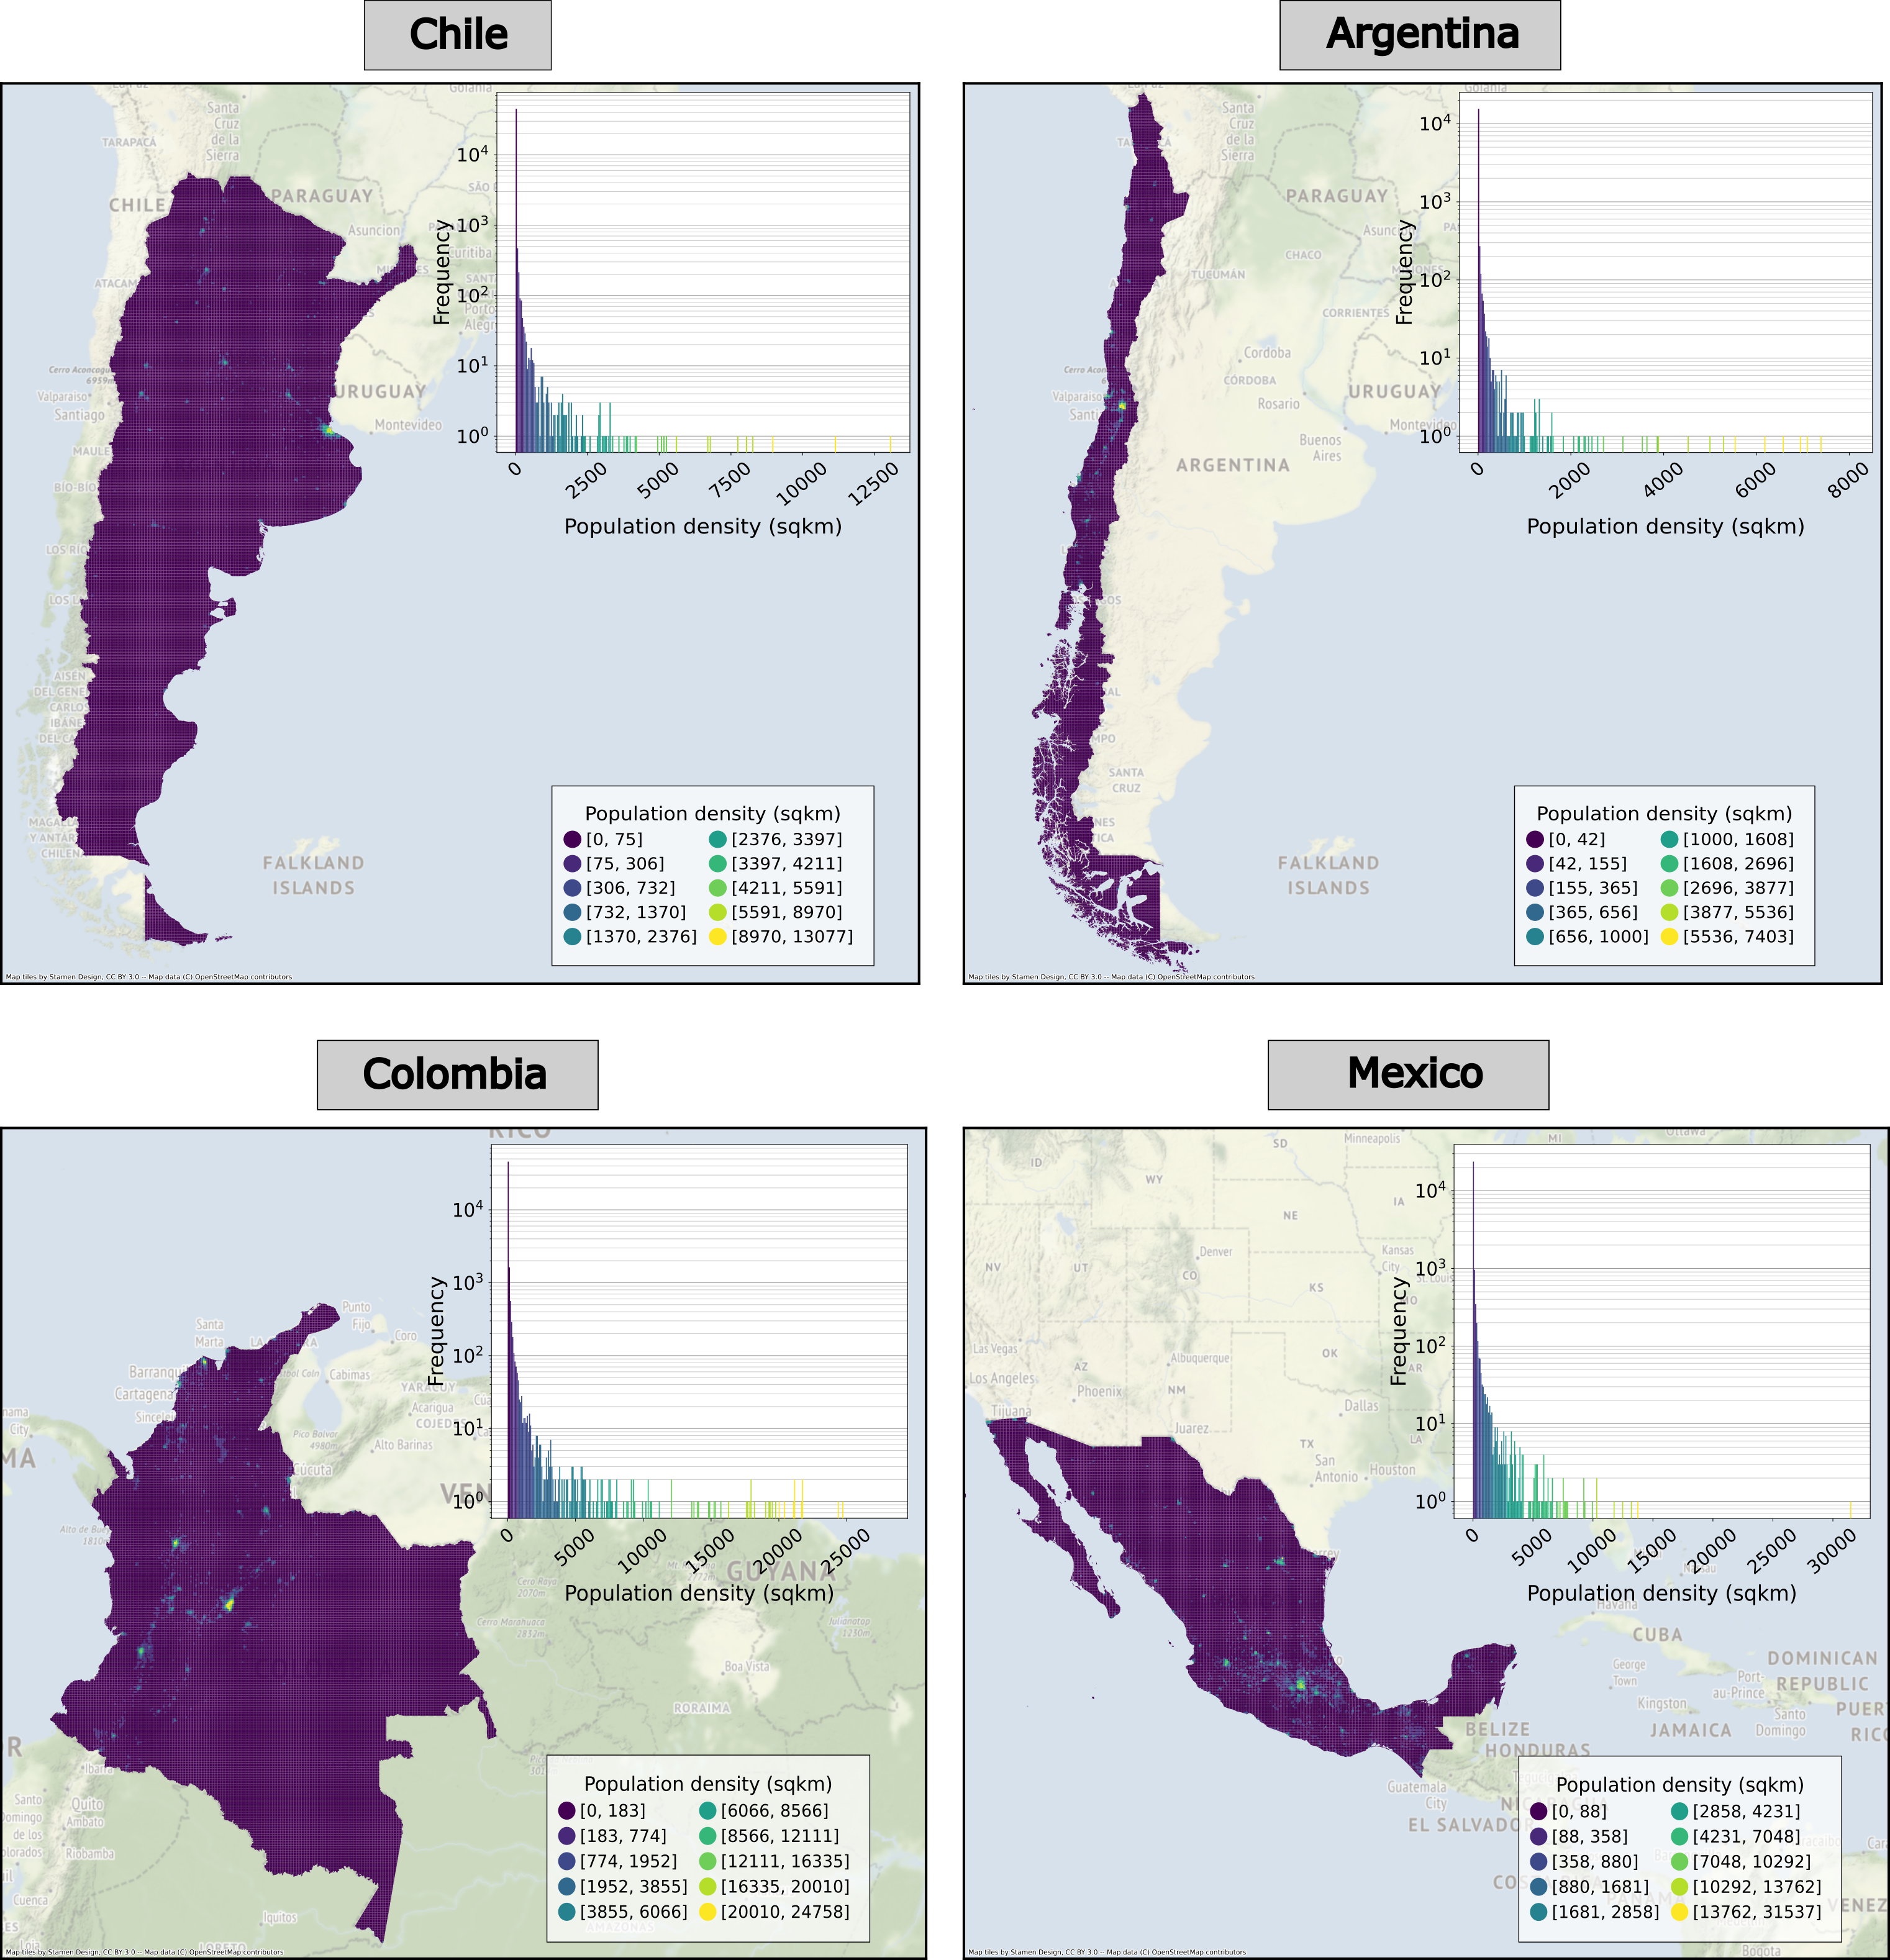
\includegraphics[width=6.51042in,height=6.66667in]{images/Map_density_histogram.png}

}

\caption{Maps of population density categories by country with
histograms, showing that the distribution of Bing tiles in each density
category.}

\end{figure}%

\subsection{Estimating the strength of the flows between tiles of different population density categories}

\ref{subsec-models}

In this section, we propose a statistical model to capture the extent to
which the strength of the population flows is systematically impacted by
the density classes of the origin and destination tiles, and how this
effect varies over time. Our approach here is very similar to that
proposed by \cite{Rowe}.

While we could obtain the population flows between different population
classes and their evolution over time, the results would fail to capture
specifically the effect of the density classes of the origin and
destination tiles. This is due to the fact that movement patterns are
influenced not only by the population density of the starting and ending
locations, but also by factors such as the distance, the population
size, the time of the week and day at which movements take place, etc.
These additional variables can act as confounding factors, obscuring the
actual impact of population density. In order to disentangle and obtain
a more accurate estimation of the importance of population density, we
chose to utilise a regression modeling approach. I AM HERE

We adopted a spatial interaction framework (Rowe, Lovelace, et al.,
2022). We used population flows between tiles by time window and day (as
described in Section 3), and modelled them as a function of
characteristics of the flow itself (Fij), the origin (Tilei) and
destination (Tilej) tiles and the temporal nature of the flow (Tw).
Crucially, we included indicator variables that capture the pair of
population classes (Figure 1) of the origin and destination tile. In
mathematical form:

\begin{enumerate}
\def\labelenumi{(\arabic{enumi})}
\setcounter{enumi}{1}
\tightlist
\item
  where µijw is the expectation of the flow of people from tile i to
  tile j in the time window w; ⍺ is an intercept; is a series of
  indicator variables that reflect the pair of population density
  classes of a given origin i (I) and destination tile j (J), resulting
  in 99 pairs (10 classes × 10 classes minus one so it is not collinear
  with ⍺); dij is the geographic distance between tiles i and j; qijw is
  a measure of the quality of the flow estimate provided by
  Meta-Facebook and related to the uncertainty behind the user count of
  the flow as described in Section 3; Popi,j represents the population
  at the origin (i) and destination (j) tiles; are parameters to
  estimate in the model linking their respective covariates to µijw; D
  is a trend tracking the day to which the flow relates to during the
  period in analysis; while Wk and H are indicator variables capturing
  day of the week (i.e., weekday or weekend) and hour window (i.e.,
  00:00--08:00, 08:00--16:00 and 16:00--00:00). Our focus in Equation
  (2) is centred on . Controlling for all other variables, these
  parameters capture the extent to which, the expected flow between a
  given origin-destination population density class pair of tiles (e.g.,
  a high-density origin to a low-density destination) is systematically
  higher or lower than if it occurred between a baseline
  origin-destination population density class pair of tiles (e.g., a
  low-density origin to a low-density destination). Additionally, we
  standardised continuous variables (dij, qijw, Popi j), α so that they
  can be interpreted as the expected flow on the first day (D = 0),
  during the first temporal window (H = 00:00--08:00), on a weekday
  (Wk = 0), for the baseline origin-population population density class
  pair, when all the other variables are at their mean value. In this
  context, each can also be seen as the `modulation factor' around that
  expectation associated with each pair of origin-destination classes.
  The baseline origin-destination population density class pair is the
  lowest population density class as origin and destination.
\end{enumerate}

We used a count data regression model. Specifically, we fitted a
generalised linear model (GLM) where the error term is assumed to be
distributed following a Poisson distribution, with a flow expectation of
(µijw) linked to the flow count (Fijw) through a log link: (3) (4) The
Poisson regression model (PRM) assumes that equidispersion, that is,
equality of mean and variance in the response variable (Cameron \&
Trivedi, 2013). In practice, the equidispersion property is commonly
violated because of overdispersion, that is, the variance exceeds the
mean. When this occurs, the PRM may produce biased parameter estimates,
causing the standard errors of the estimates to be underestimated, and
compromising the statistical inference process (Hilbe, 2011). To test
for overdispersion, we used a regression-based test based on an
auxiliary regression of the conditional variance as described in Cameron
and Trivedi (2013).

Following Gelman and Hill (2006), we used a quasi-PRM to address
overdispersion in our response variable. This is one of the most common
strategies to deal with overdispersion in count data models (Hilbe,
2011). Intuitively, this model adjusts the standard errors of the
estimates to account for the extra dispersion in the data. To implement
this, we estimated Equation (2) by using robust variance estimators. The
number of active Facebook users were used as a weight to account for the
variability of the observed count of population movement over time. This
strategy is also used to mitigate for any potential biases regarding the
variation in the observed number of active Facebook users changes over
time across Britain.

We fitted Equation (2) using iteratively reweighted least squares
(IWLS). We separately estimated models for individual months in our
data, resulting in 18 sets of estimates. Our key aim was to generate
estimates for ⍺ and , so that we focused on discussing the evolution of
these estimates in a grid of line plots with 10 rows and 10 columns,
each of them representing one of our population density classes. The
plot corresponding to the Ith row and Jth column displays the evolution
of the parameter that tracks the intensity of population flows from
tiles in population density class Ith to those in population density
class Jth.

\section{Results}\label{sec-results}

\section{Discussion}

\section{Conclusion}

\section{References}

\phantomsection\label{refs}
\begin{CSLReferences}{1}{0}
\bibitem[\citeproctext]{ref-Maas19}
Maas, P., S. Iyer, A. Gros, W. Park, L. McGorman, C. Nayak, and P. A.
Dow. 2019. {``Facebook Disaster Maps: Aggregate Insights for Crisis
Response and Recovery.''} In \emph{16th International Conference on
Information Systems for Crisis Response and Management}, 836--47.

\bibitem[\citeproctext]{ref-rowe2022}
Rowe, Francisco, Alessia Calafiore, Daniel Arribas-Bel, Krasen
Samardzhiev, and Martin Fleischmann. 2022. {``Urban Exodus?
Understanding Human Mobility in Britain During the COVID-19 Pandemic
Using Facebook Data.''} \url{https://doi.org/10.48550/ARXIV.2206.03272}.

\bibitem[\citeproctext]{ref-wang2022}
Wang, Yikang, Chen Zhong, Qili Gao, and Carmen Cabrera-Arnau. 2022.
{``Understanding Internal Migration in the UK Before and During the
COVID-19 Pandemic Using Twitter Data.''} \emph{Urban Informatics} 1 (1).
\url{https://doi.org/10.1007/s44212-022-00018-w}.

\end{CSLReferences}




% print the bibliography
\setlength{\bibsep}{0.00cm plus 0.05cm} % no space between items
\bibliographystyle{apalike}
\bibliography{sim_refs}



\end{document}
